\section{Estimación de Variables Peatonales}

Nuestro objetivo es estimar y calcular ciertas métricas por período de tiempo
(el cálculo es posible hacerlo por hora, por día, por semana).
Hemos priorizado en las definiciones de las variables peatonales 
y métodos de cálculo que se garantice la coherencia interna, en otras palabras
dado un período de tiempo que empieza y termina con el local vacío.

%\subsection{Definiciones}

Sean $V_T$ las visitas totales, $\overline{Oc}$ y $\overline{Tp}$ 
la ocupación y el tiempo de permanencia promedios durante el período $T$

\begin{equation} 
   \frac{\overline{Oc}}{\overline{Tp}} = \frac{V_T}{T}
   \label{eq:OcTpVT}
\end{equation}

\subsection{Circulación exterior en el pasillo}
La circulación exterior $C$ la detectamos con un sensor Clarity ubicado en el pasillo,
considerando el Área del local $L$ y el Área de detección donde está incluí­do $A$, $L \subset A$,
la cantidad de personas $P = C + V = (1 + \gamma)C$ donde $\gamma$ es el coeficiente de tracción del local
en el Área $A$ para estimación el factor de detección $f$.
Sea $p$ un umbral, cota inferior, de potencia máxima; llamamos $f^p$ al factor estimado usando $M\big|^{\ge p}$,
$f_{5}^p$ y $f_{95}^p$ a los respectivos percentiles 5 y 95,
es decir, eliminando el 5\% de outlyers en ambos extremos.
\[
= \bar{f} = \min_p \frac{f_{95}^p - f_5^p}{f^p}
\frac{M_A}{(1 + \gamma)C} 
\le \frac{M_A}{C} = f^A_C 
\]
que minimice su error relativo, obteniéndose así un
estimador de la cota superior para el factor $f$ de detecciones en el Área $A$,
donde $p$ es la potencia máxima detectada por el cluster para incluirlo en $M_A$. 

\subsection{Resultados}

\begin{table}[]
\centering
\caption{optimización de coef. corr. y rango relativo de $f$}
\label{tab:opt}
\begin{tabular}{|l|l|ll|ll|}
\hline
$p$   & Corr     & cota inferior & cota superior & $f$        & rango relativo \\
\hline
-80 & 0.624377 & 0.492911      & 0.935338      & 0.741483 & 0.596678       \\
-79 & 0.641995 & 0.480378      & 0.881847      & 0.704438 & 0.569915       \\
-78 & 0.652574 & 0.467434      & 0.832009      & 0.670504 & 0.543733       \\
-77 & 0.667754 & 0.454695      & 0.785177      & 0.638116 & 0.517903       \\
-76 & 0.684607 & 0.443600      & 0.741783      & 0.608435 & 0.490082       \\
-75 & 0.694458 & 0.430450      & 0.702256      & 0.580481 & 0.468242       \\
-74 & 0.702606 & 0.418122      & 0.664662      & 0.552583 & 0.446159       \\
-73 & 0.715276 & 0.404561      & 0.609237      & 0.520184 & 0.393468       \\
-72 & 0.722541 & 0.389357      & 0.564075      & 0.487673 & 0.358269       \\
-71 & 0.740117 & 0.373125      & 0.523962      & 0.458825 & 0.328746       \\
-70 & 0.745787 & 0.357304      & 0.485623      & 0.431512 & 0.297370       \\
-69 & 0.761884 & 0.344976      & 0.448704      & 0.403891 & 0.256821       \\
-68 & 0.772981 & 0.325457      & 0.414982      & 0.375372 & 0.238496       \\
\textbf{-67} & 0.775064 & 0.308923      & 0.387471      & 0.350115 & \textbf{0.224349}       \\
-66 & 0.780560 & 0.284000      & 0.364269      & 0.324733 & 0.247185       \\
-65 & 0.788781 & 0.260308      & 0.339079      & 0.300629 & 0.262021       \\
-64 & 0.797413 & 0.239385      & 0.314219      & 0.275788 & 0.271349       \\
-63 & 0.804507 & 0.212923      & 0.286046      & 0.250610 & 0.291778       \\
-62 & 0.797379 & 0.192000      & 0.257755      & 0.224734 & 0.292590       \\
-61 & 0.785839 & 0.165846      & 0.228041      & 0.198663 & 0.313068       \\
-60 & 0.788161 & 0.146462      & 0.199509      & 0.172974 & 0.306679       \\
-59 & 0.781836 & 0.128000      & 0.171837      & 0.148499 & 0.295198       \\
-58 & 0.771302 & 0.107692      & 0.144164      & 0.125416 & 0.290809       \\
-57 & 0.768602 & 0.083385      & 0.121625      & 0.103420 & 0.369754       \\
-56 & 0.750365 & 0.070462      & 0.099437      & 0.086040 & 0.336762       \\
-55 & 0.763828 & 0.057538      & 0.083195      & 0.071529 & 0.358692       \\
-54 & 0.740633 & 0.048309      & 0.070600      & 0.059040 & 0.377555       \\
-53 & 0.680608 & 0.038345      & 0.058999      & 0.049282 & 0.419087       \\
-52 & 0.657073 & 0.032005      & 0.052038      & 0.041120 & 0.487203       \\
\hline
\end{tabular}
\end{table}

El método que utilizamos fue un método de umbral (threshold) que selecciona utiliza la para seeccionar una detección válida que potencia máxima del cluster sea superior a un cierto valor. Para encontrar ese valor usamos dos estrategias, una es ver cual tenia máxima correlación, o sea, que la cantidad de cluster que superen ese valor maximizaba esa correlación con la circulación que se medía con el sensor de clarity de la circulación en el pasillo.
El otro criterio fue elegir el valor de $p$ que minimizara el error relativo, 
excluimos el 5\% superior y el 5\%inferior de la muestra y calculamos esos percentiles. 
El percentil 95 menos el percentil 5 y dividimos el valor del factor calculado, el valor calculado es qué cantidad de cluster se detectan.
La metodología fue seleccionar 21 días para mantener la igual proporción de días hábiles y fines de semana, excluimos la semana de la promoción dado que esto podría alterar el comportamiento. Con estos 21 días calculamos el factor y lo utilizamos  para predecir los días siguientes

La Figura~\ref{fig:fitting_67} se ve los valores del factor y los errores tantos al 100\% 
como al 95-vo y el 5-to percentil

\begin{figure}[H] 
  \centering
  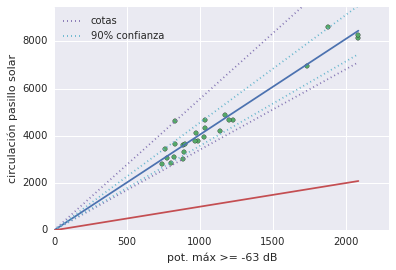
\includegraphics[width=0.5\textwidth]{Fig_fit_circulacion_por_jornada.png}
  \caption{
  sample size = 21, $p$ = 67
coef.corr.($s, c_p$) = 0.789206
$f$ = 0.339301, estimador de detección $f = 1/b$ asumiendo fitting $y = b x$
inf = 0.241768, sup = 0.414193, rango rel. = 0.508179
$f_5$ = 0.294769, $f_{95}$ = 0.373550, rango rel. = 0.232185
  }
  \label{fig:fitting_67}
\end{figure}

En la Figura~\ref{fig:prediction} podemos como como los valores que no estaban en la muestra: los valores que se tomaron después (los puntos) rojos no caen en el cono donde esperábamos que deberían caer.

\begin{figure}[H] 
  \centering
  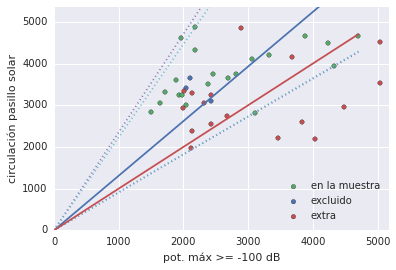
\includegraphics[width=0.5\textwidth]{scatter-sample-n-next.png}
  \caption{valores medidos después de la muestra de 21 días tienen color rojo
  }
  \label{fig:prediction}
\end{figure}

\[
f = \frac{M_A \Big|_{t\ge 0}^{p \ge -67dB}}{C}
\]


Mediante el resultado de un estudio de 21 jornadas,
obtuvimos $\bar{f} = 0.35$ con confianza de $\beta = 0.90$,
eliminando los outlyers del 5to y 95vo percentil,
$0.31 \le \bar{f} \le 0.38$. Dando un error relativo 
\[
\frac{\bar{f}_{95}^p - \bar{f}_5^p}{\bar{p}} = 0.22
\]

Si analizamos la Figura~\ref{fig:prediction} donde vemos la relación entre la medición de los cluster y la relación con los clarity, vemos que la nube de puntos correspondientes a la circulación medida por el sensor Clarity se mantiene en los mismos rangos, mientras que la nube de puntos de la medición del los urbix-nodos se aparta de ese rango. La distribución de los cluster pierde correlación.

Aparentemente la distribución de circulación cambia para los nuevos días pero
las detecciones de los nodos se mantienen dentro de los rangos que estaban. Los valores que 
fueron excluidos (en azul) debido a las promociones, están dentro del cono de predicción. Sin embargo los correspondientes a mediciones posteriores, no. Esto puede deberse a que hubo un cambio de situación. O que el algoritmo no está ignorando factores de estacionalidad.


\subsection{Visitas}
Nuestra definición de visitas, se basa en personas q ingresan por más de 30 segundos
por lo que usamos $t \ge 30$ segundos. Para calcular el umbral de potencia máxima $p$
usamos los datos anteriores como cota inferior o subestimador, 
ya que la problemática de un pasillo se asume que el factor de detección en el mismo 
es menor que al factor de detección de un local donde la gente permanece más tiempo en el

\[
\bar{f} \le f^L_d = f^L = \frac{M_L}{V} \le f^A
\]
Se puede tomar como cota superior el valor que se 
obtiene del valor mínimo observado 
$\widetilde{f^L} = \min_i M_i/C_i$ sin aplicarle ningún filtro
lo que nos da el supremo (la mínima cota superior)
durante los días de la muestra que es $0.60$ como se observa en la Figura~(\ref{fig:CotaSup})

\begin{figure}[H] 
  \centering
  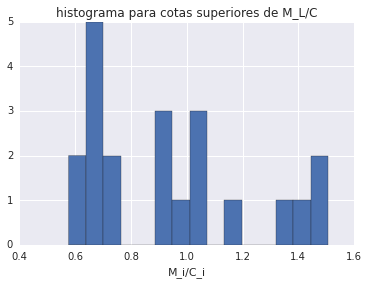
\includegraphics[width=0.5\textwidth]{cota_sup_hist.png}
  \caption{
    histograma de las posibles cotas superiores de $\frac{M_L}{V},
    \min_i \frac{M_i}{C_i} = 0.576125$
  }
  \label{fig:CotaSup}
\end{figure}

Vamos a tomar como factor de detección para la problemática del local $f$
como un valor entre la cota inferior $\bar{f}_{95}$,
y la superior,
\[
\bar{f}_{95} \le f_L \le \widetilde{f}
\],
para el caso vamos a tomar el promedio
$f_L = (0.38 + 0.60)/2 = 0.44$.

\paragraph{Algoritmo}
Para calcular o estimar las visitas $V$
escogimos el umbral $\bar{p}$ para construir un filtro de detecciones
\[
\frac{M_L \Big|_{t\ge 30}^{p \ge \bar{p}}}{V} \simeq \bar{f}
\]
que ajuste a los valores medidos in situ.
\[
V = \bar{f} M \Big|_{t \ge 30}^{p \ge \hat{p}}
\]


\begin{figure}[H] 
  \centering
  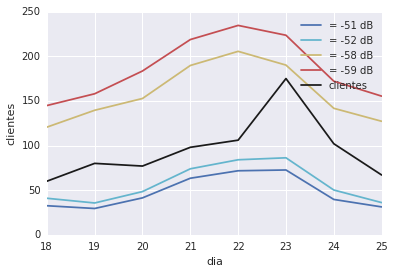
\includegraphics[width=0.5\textwidth]{cotas_sup_inf_valores_diarios_pot_conteos.png}
  \caption{
    calibración de visitas por hora tomados por empleados
  }
  \label{fig:mediciones_cotas}
\end{figure}

Las Figuras~\ref{fig:mediciones_cotas}~y~\ref{fig:mediciones_intermedios} muestran cómo se comporta la estimación de la visitas usando $\bar{p}$ mayor a los usados en el pasillo, ya que se espera que los clusters detectados dentro del local tengan mayor intensidad.  

\begin{figure}[H] 
  \centering
  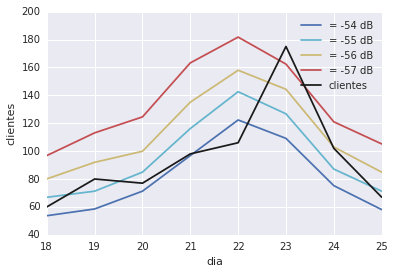
\includegraphics[width=0.5\textwidth]{pot_que_no_estiman_correctamente_los_conteos.png}
  \caption{
    potencias con valores intermedios a las cotas. 
  }
  \label{fig:mediciones_intermedios}
\end{figure}
Se observa un outlayer el 13/4/16 que no puede ser explicado por este método.

Se están recolectando más datos que tomando por los empleados. Esos datos nos van a permitir calcular un mejor estimador de visitas diarias. El grado de precision que podemos trabajar es a nivel de día, dado que a nivel hora, el margen de error es muy grande.
Sin embargo, La Figura~\ref{fig:estimacion_x_hora} muestra que existe una buena correlación entre el promedio de la hora y el valor medido.
Es una medición similar al la estimación de circulación pero en vez de estar midiendo con un sensor clarity estamos usando una medición manual de los empleado. Así mismo debemos considerar que ésta forma de recaudar información a través de los empleados es un subestimador de gente que entra en la visita, porque generalmente los empleados van a contar de menos y no de más.
Con esos datos investigamos un valor de umbral para asignar los cluster que superen ese valor de potencia máxima.

Nuestra definición de visitas (ejemplo: se basa en personas q ingresan por más de 30 sec).
Para la estimación del error de nuestro método, se necesita contar con más muestras in situ.
Este método de selección de cluster a usando un umbral parece ser sensible a casos especiales. Vamos a desarrollar a continuación una o familia de algoritmos para resolver esta cuestión. Los resultados se mostrarán en el próximo informe.

\begin{figure}[H] 
  \centering
  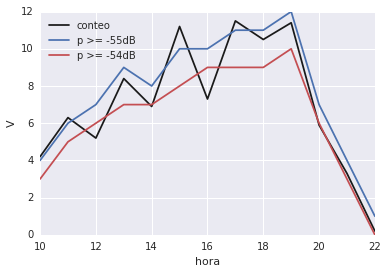
\includegraphics[width=0.5\textwidth]{pot_para_est_x_hora.png}
  \caption{
    potencias con valores intermedios a las cotas. 
  }
  \label{fig:estimacion_x_hora}
\end{figure}

La Figura~\ref{fig:estimacion_x_hora} muestra que para una estimación de la distribución de visitas según la hora, seleccionar unos valores de potencia máximas mayores o iguales a $\bar{p} = -55$ o $\bar{p} = -54$ provee una buena aproximación.


\subsection{ocupación y tiempo de permanencia}
Nuestra definición de ambas variables
sigue las mismas pautas que para la variable visitas (ejemplo: se basa en personas que ingresan por más de 30 sec) 

El cálculo de estas 3 variables tanto por jornada
como por hora,
se realiza a través de las visitas y funciones sql
La ocupación promedio es medida usando ponderación de tiempo de permanencia, y tiene  coherencia interna entre el tiempo de permanencia y la ocupación según la formula 

\section{Próximos pasos}

\subsection{Histogramas de potencias máximas}
En el próximo reporte vamos a analizar diferentes perfiles de distribución frecuencias de potencias máximas detectadas y presentar una nueva familia de algoritmos basada en el filtrado de curvas de distribución superpuestas. He aquí una muestra de los diferentes tipos de distribuciones que encontramos.

\begin{figure}[H] 
  \centering
  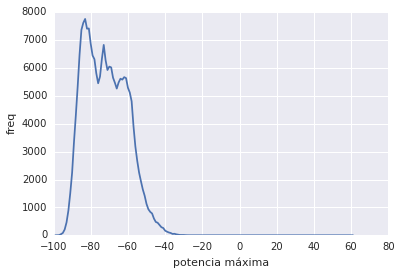
\includegraphics[width=0.5\textwidth]{pot_max.png}
  \caption{distribución de potencias máximas}
  \label{fig:pot_max_total}
\end{figure}

\begin{figure}[H] 
  \centering
  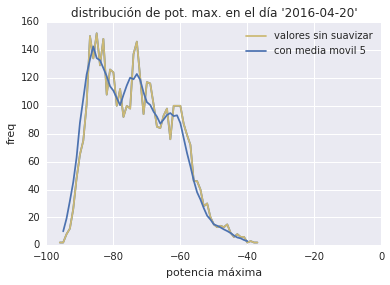
\includegraphics[width=0.5\textwidth]{pot_max_2016-04-20.png}
  \caption{distribución de potencias máximas de un solo día: el dia 20 de abril}
  \label{fig:pot_max_1_dia}
\end{figure}

\begin{figure}[H] 
  \centering
  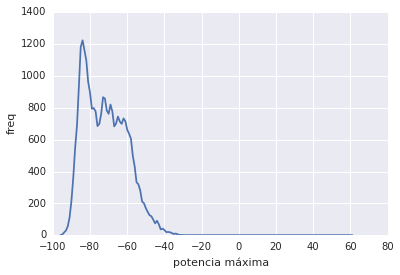
\includegraphics[width=0.5\textwidth]{pot_max_2016-04-10_al_16.png}
  \caption{distribución de potencias máximas de una semana: del 10 al 16/4}
  \label{fig:pot_max_semana}
\end{figure}

\begin{figure}[H] 
  \centering
  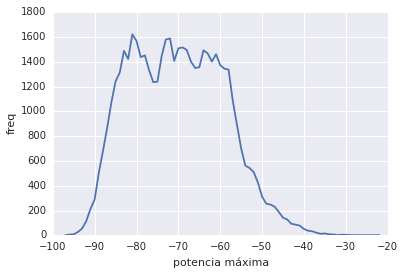
\includegraphics[width=0.5\textwidth]{pot_max_muestra.png}
  \caption{distribución de potencias máximas de la muestra}
  \label{fig:pot_max_muestra}
\end{figure}

\begin{figure}[H] 
  \centering
  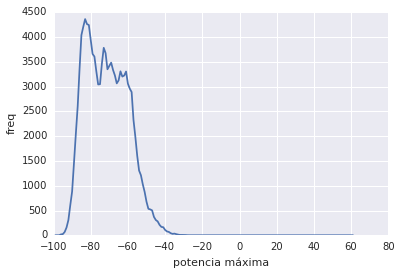
\includegraphics[width=0.5\textwidth]{pot_max_mes.png}
  \caption{distribución de potencias máximas de un mes: del 15/3 al 14/4}
  \label{fig:pot_max_mes}
\end{figure}




